\documentclass[12pt,a4paper]{scrartcl}
    \usepackage[utf8]{inputenc}
    \usepackage{amsmath}
    \usepackage{amsfonts}
    \usepackage{amssymb}
    \usepackage{graphicx}

    \usepackage[bottom = 1in, left = 0.5in, right = 0.5in, top = 1in]{geometry}

    \usepackage[english]{babel}
    \usepackage[autostyle]{csquotes}
    \usepackage{mathptmx}

    \usepackage[labelfont=bf]{caption}

    \usepackage[default, scale=0.95]{opensans}

    \usepackage[T1]{fontenc}

	\usepackage{fixltx2e}
	
	\usepackage{textcomp}

    % \addto\captionsenglish{\renewcommand{\figurename}{Supplementary Fig.}}
    % \addto\captionsenglish{\renewcommand{\tablename}{Supplementary Table}}

    \title{Figures}
    \date{}

\begin{document}
\maketitle

\begin{figure}[h]
	\centering
	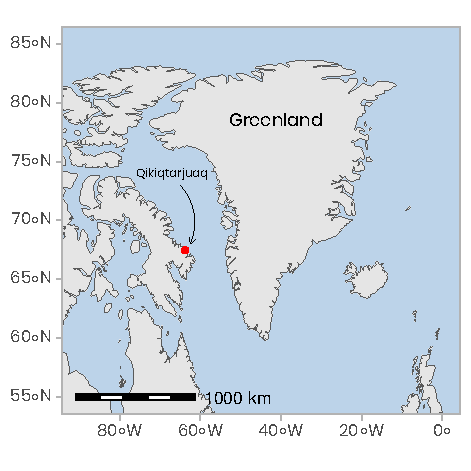
\includegraphics[scale = 1]{../../../graphs/fig01.pdf}
	\caption{Location of the ice camp located near the Qikiqtarjuaq Island in the Baffin Bay. Projection used: EPSG-4326.}
\end{figure}

\clearpage
\newpage

\begin{figure}[h]
	\centering
	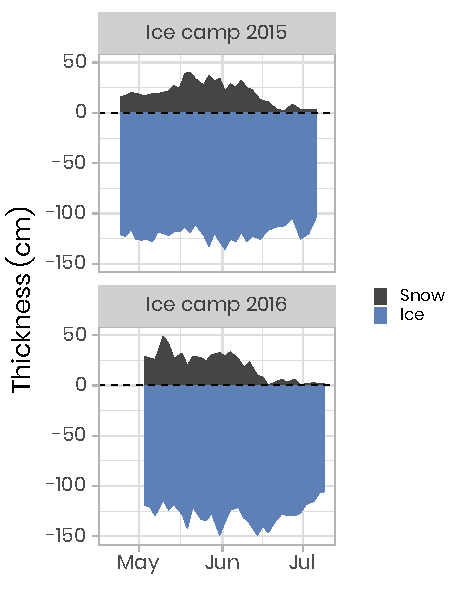
\includegraphics[scale = 1]{../../../graphs/fig02.pdf}
	\caption{Temporal evolution of the snow and sea-ice thickness for both ice camp missions. The dashed horizontal line represents the snow/ice interface.}
\end{figure}

\clearpage
\newpage

\begin{figure}[h]
	\centering
	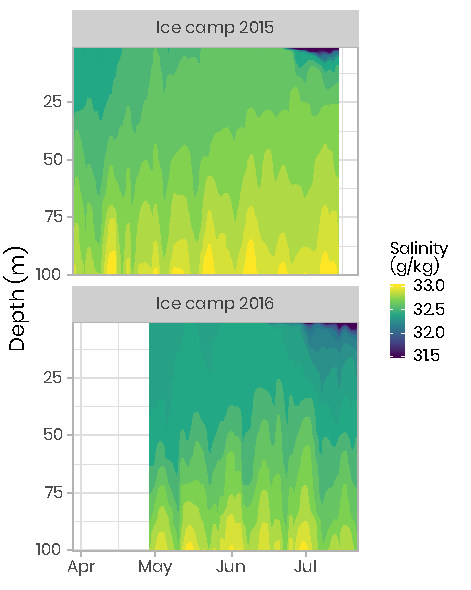
\includegraphics[scale = 1]{../../../graphs/fig03.pdf}
	\caption{Temporal evolution of the salinity in the first 100 meters of the water column for both campaigns. Note that for visualization, salinity below 31.5 g kg\textsuperscript{-1} have been binned to 31.5 g kg\textsuperscript{-1}.}
\end{figure}

\clearpage
\newpage

\begin{figure}[h]
	\centering
	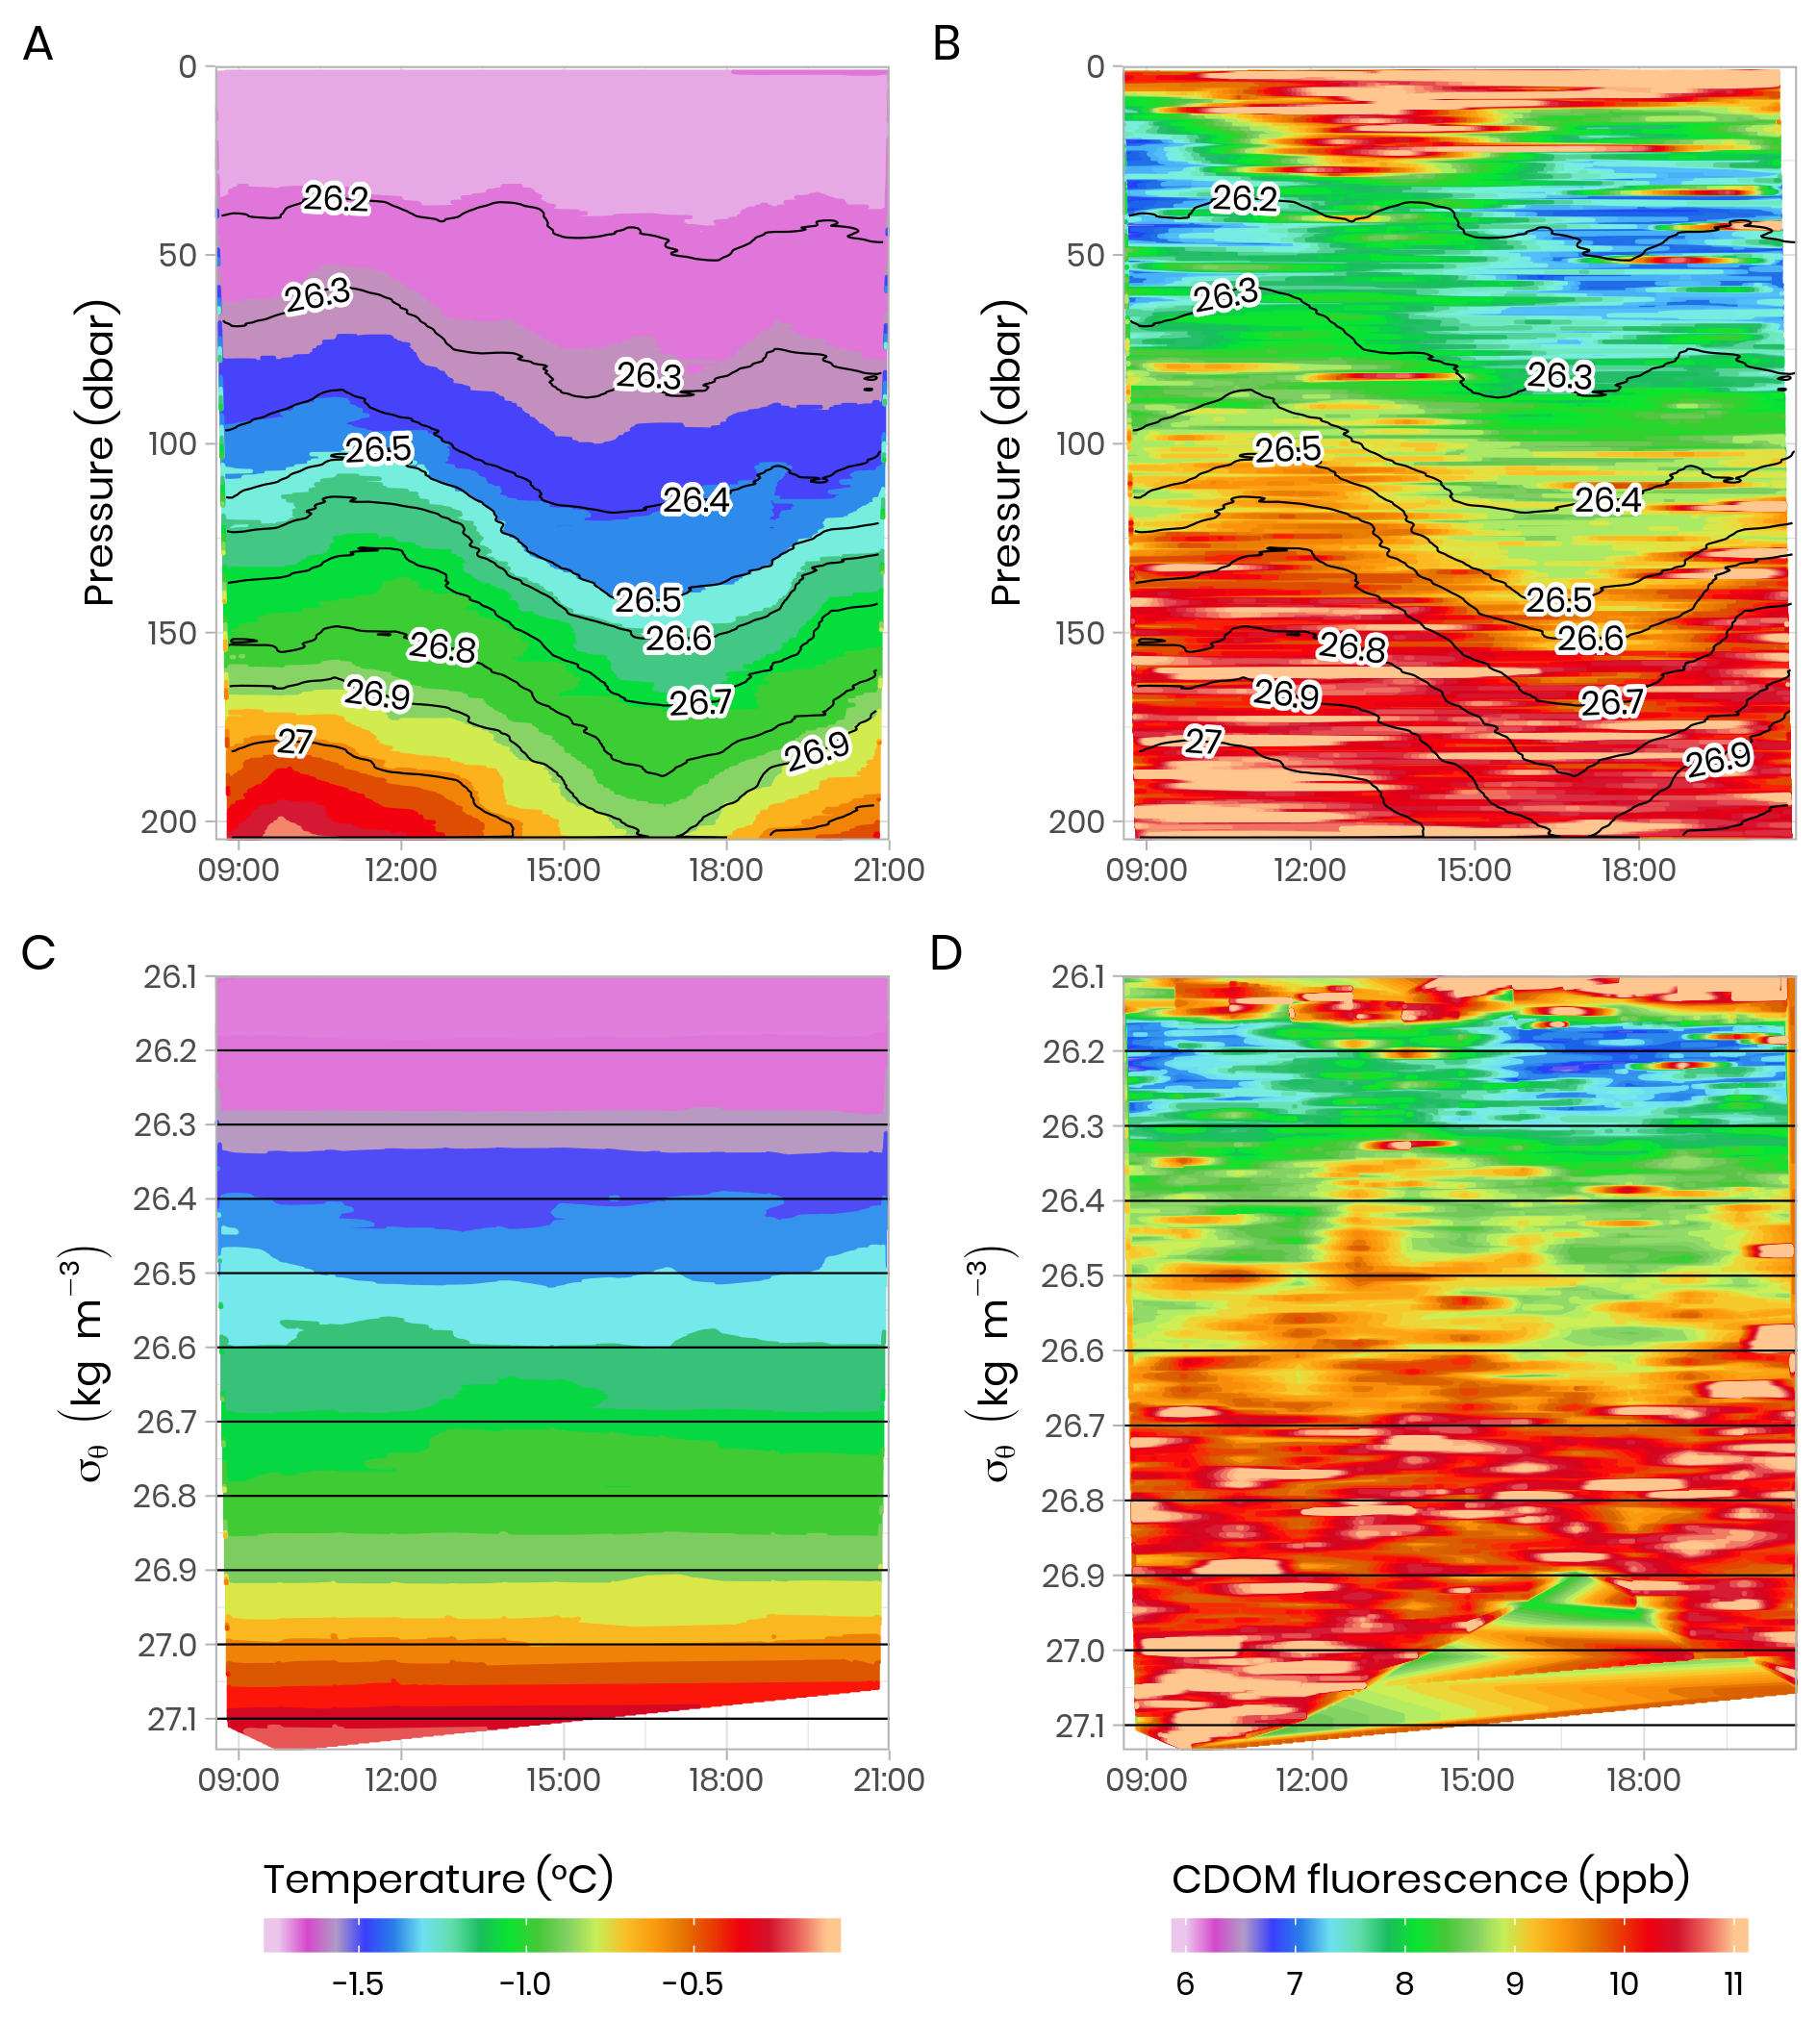
\includegraphics[scale = 1]{../../../graphs/fig04.png}
	\caption{Temporal evolution of physical (temperature) and bio-optical (CDOM fluorescence) variables with superimposed lines of potential density anomaly ($\sigma_\theta$, kg m\textsuperscript{-3}) during a 13-h tidal cycle. Surface tidal height versus time at Qikiqtarjuaq is shown in blue. (A-B) Plotted versus pressure coordinates (equivalent to depth in meters). (C-D) The same data plotted versus potential density anomaly $\sigma_\theta$ coordinates (kg m\textsuperscript{-3}). The tidal survey was performed on 2015-06-09.}
\end{figure}

\begin{figure}[h]
	\centering
	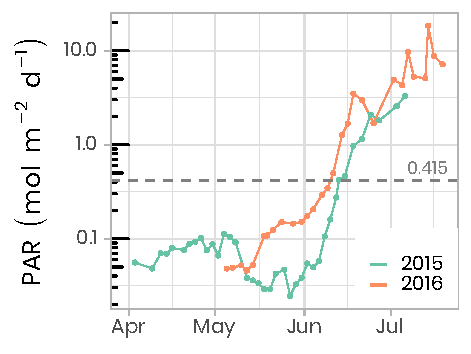
\includegraphics[scale = 1]{../../../graphs/fig05.pdf}
	\caption{Temporal evolution of daily photosynthetically available radiation (PAR) at the sea-ice/water interface (1.3 m depth) for both ice camp missions. The horizontal dashed line shows the 0.415 mol photons m\textsuperscript{-2} d\textsuperscript{-1} threshold often used in the literature as the minimum light requirement for primary production.}
\end{figure}

\clearpage
\newpage

\begin{figure}[h]
	\centering
	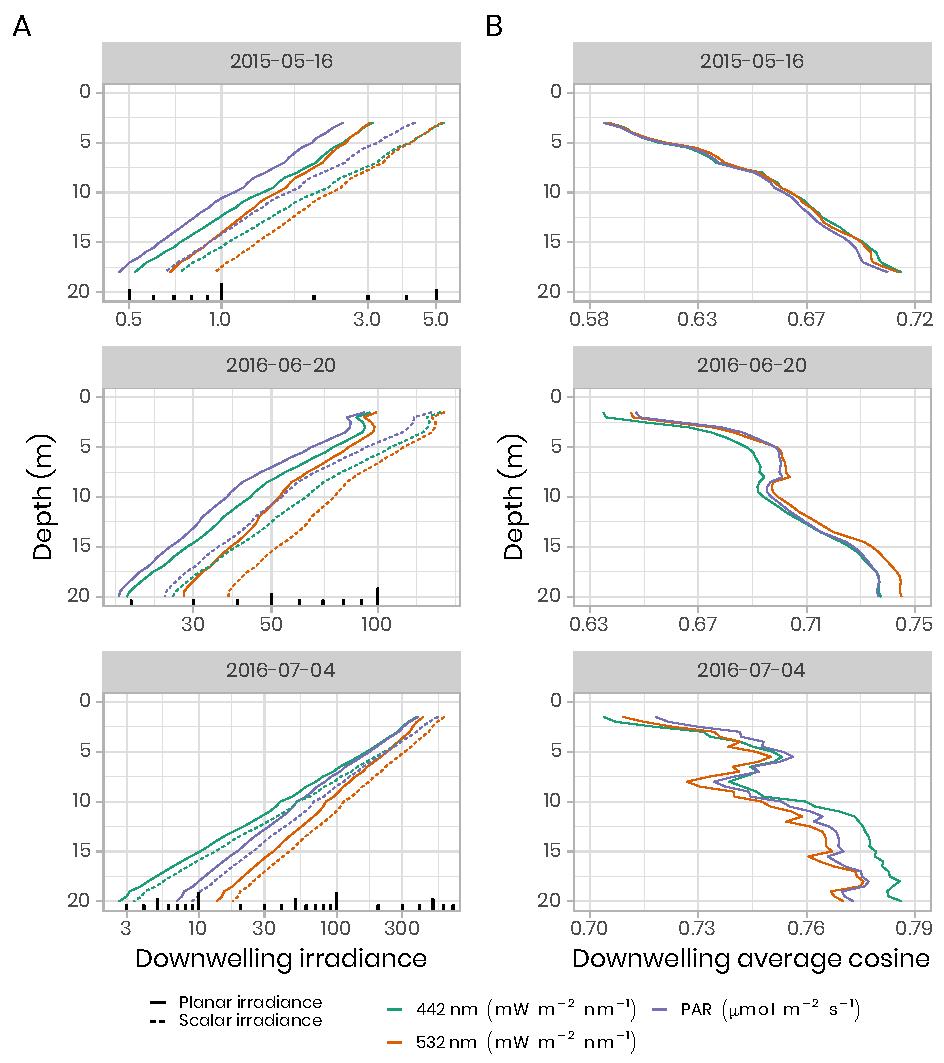
\includegraphics[scale = 1]{../../../graphs/fig06.pdf}
	\caption{(A) Under-ice vertical profiles of downwelling planar and scalar irradiance at 442 nm, 532 nm and for PAR. (B) Calculated downwelling average cosine (unitless) was measured beneath snow-covered sea ice on 16 May 2015, beneath bare ice on 20 June 2016 and beneath a melt pond on 4 July 2016. Note the log scale for the irradiance measurements (A).}
\end{figure}

\clearpage
\newpage

\begin{figure}[h]
	\centering
	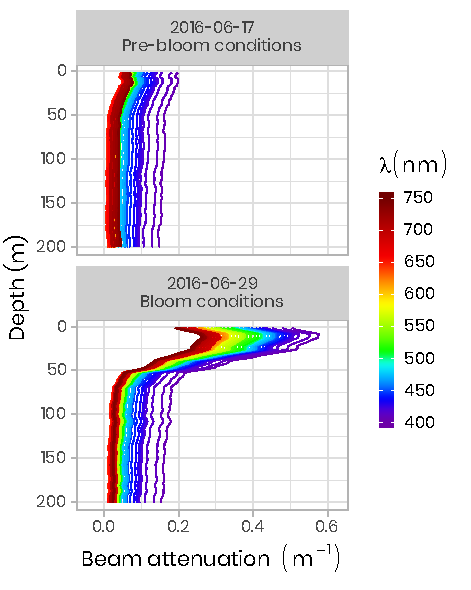
\includegraphics[scale = 1]{../../../graphs/fig07.pdf}
	\caption{Beam attenuation coefficients ($c$, m\textsuperscript{-1}) measured in 2016 using an ACS before and during the phytoplankton bloom. Note that the colors of the lines correspond to wavelength frequencies.}
\end{figure}

\clearpage
\newpage

\begin{figure}[h]
	\centering
	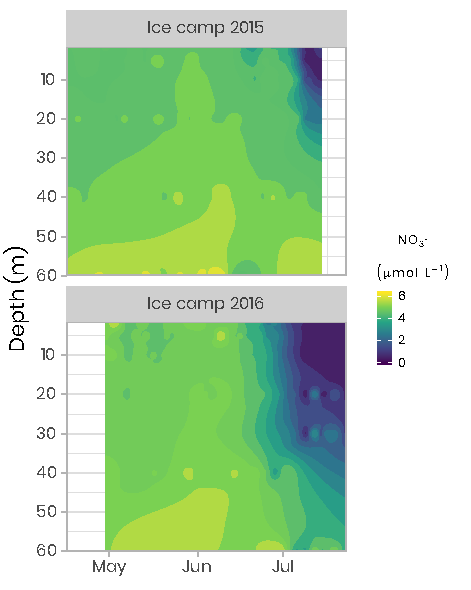
\includegraphics[scale = 1]{../../../graphs/fig08.pdf}
	\caption{Temporal evolution of the nitrates in the first 60 m of the water column for both ice camp missions.}
\end{figure}

\clearpage
\newpage

\begin{figure}[h]
	\centering
	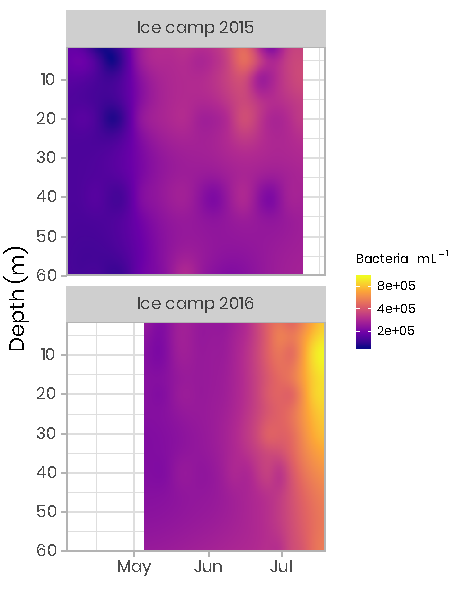
\includegraphics[scale = 1]{../../../graphs/fig09.pdf}
	\caption{Concentration of bacteria in the water column at the ice camp in 2015 and 2016.}
\end{figure}

\clearpage
\newpage

\begin{figure}[h]
	\centering
	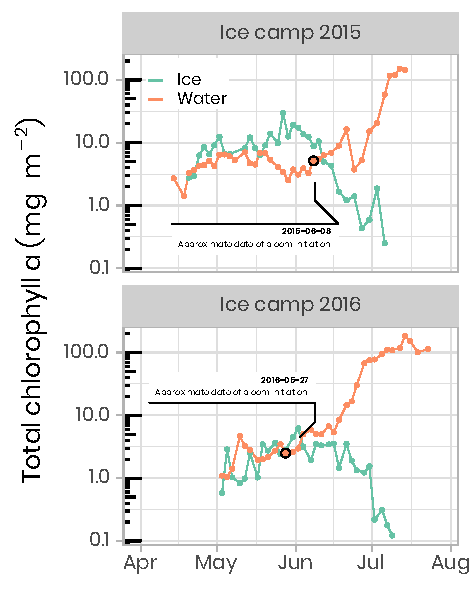
\includegraphics[scale = 1]{../../../graphs/fig10.pdf}
	\caption{Temporal evolution of chlorophyll a in ice and water (depth-integrated) for both ice camp missions. Note that the water chlorophyll a have been integrated over the first 100 m of the water column whereas the ice chlorophyll a was measured on the bottom 0-10 cm of the ice cores. The details of the calculations to determine the approximate dates of phytoplankton bloom initiation can be found in Oziel et al. (2019).}
\end{figure}

\clearpage
\newpage

\begin{figure}[h]
	\centering
	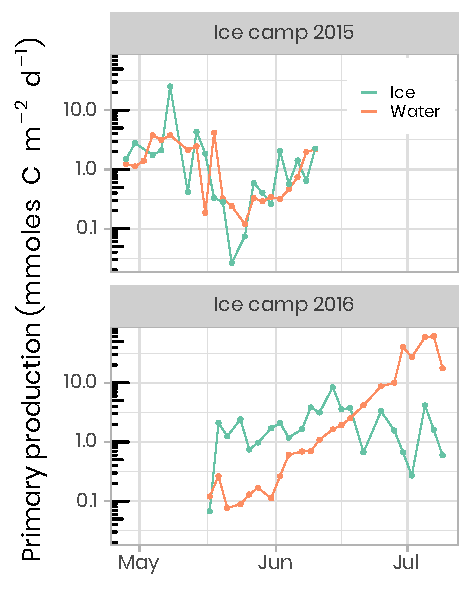
\includegraphics[scale = 1]{../../../graphs/fig11.pdf}
	\caption{Temporal evolution of primary production a in ice and water (depth-integrated) for both ice camp missions.}
\end{figure}

\clearpage
\newpage

\begin{figure}[h]
	\centering
	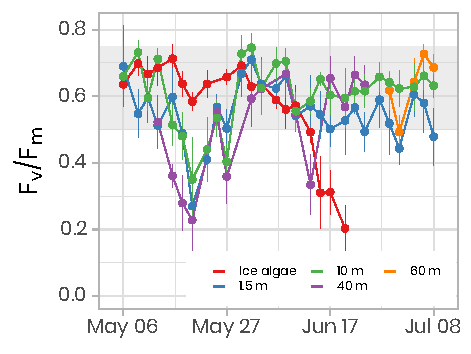
\includegraphics[scale = 1]{../../../graphs/fig12.pdf}
	\caption{Images of protists sampled with the IFCB. Scale bar on images is 10 µm. Note that images are not to scale. (\textbf{A}) \textit{Anabaena} sp. (\textbf{B}) \textit{Nitzschia frigida} (\textbf{C}) \textit{Polarella glacialis} (\textbf{D}) Flagellate (\textbf{E}) Euglena (\textbf{F}) \textit{Pseudo-nitzschia} sp. (\textbf{G}) \textit{Ceratium} sp. (\textbf{H}) \textit{Thalassiosira nordenskioeldii} with \textit{Attheya septentrionalis} (\textbf{I}) \textit{Peridiniella catenata} (\textbf{J}) \textit{Navicula pelagica} (\textbf{K}) \textit{Phaeocystis} sp. colony (\textbf{L}) \textit{Chaetoceros} sp. (\textbf{M}) \textit{Entomoneis} sp. (\textbf{N}) \textit{Synedropsis hyperborea} (\textbf{O}) Ciliate (\textbf{P}) Pennate diatom (\textbf{Q}) \textit{Eucampia} sp. (\textbf{R}) \textit{Melosira} sp.}
\end{figure}

\clearpage
\newpage

\begin{figure}[h]
	\centering
	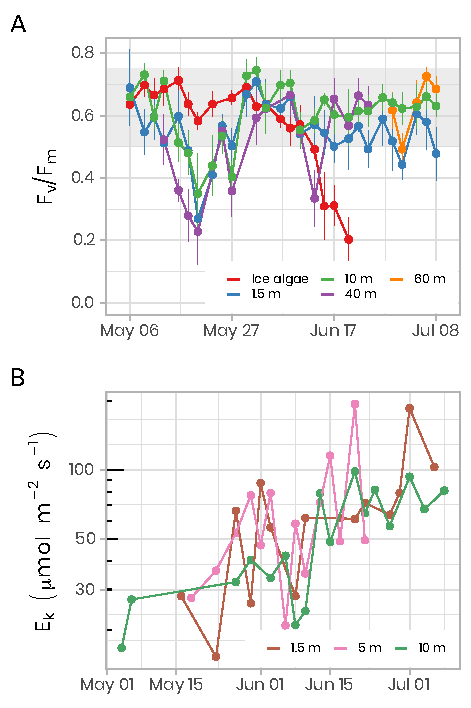
\includegraphics[scale = 1]{../../../graphs/fig13.pdf}
	\caption{Temporal evolution of $F_v/F_m$ for ice (last cm) and water underneath the ice (depths 1.5 m, 10 m, 40 m) samples for the ice camp 2016 between May 6\textsuperscript{th} and July 8\textsuperscript{th}. $F_v/F_m$ monitoring on ice samples stopped on Day 172-June 20th because the Chl a fluorescence signal was not reliable anymore. $F_v/F_m$ monitoring on 40 m and 60 m depth samples was limited between May 13th and June 24th and between June 29th-July 08th, respectively. The gray shaded area represents the range at which the algae are optimally growing.}
\end{figure}

\clearpage
\newpage

\begin{figure}[h]
	\centering
	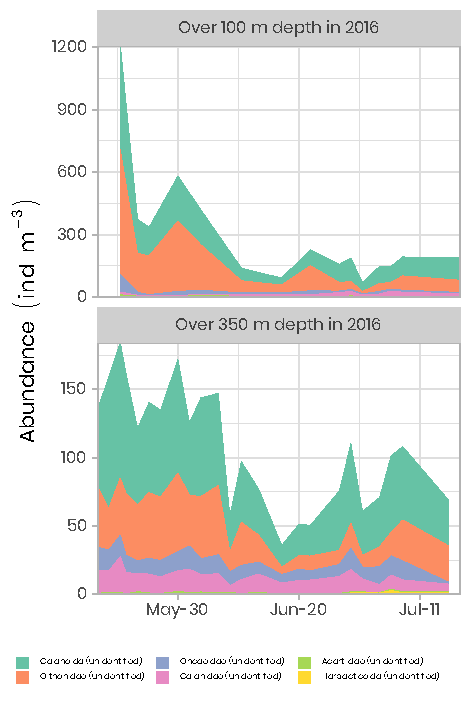
\includegraphics[scale = 1]{../../../graphs/fig14.pdf}
	\caption{Time series of the abundance of the copepods (ind m\textsuperscript{-1}) measured over the first 100 m and 350 m of the water column in 2016 using the zooscan. For visualization, only the six most abundant groups are presented in decreasing order of importance. Note the different y-axes in both panels.}
\end{figure}

\end{document}
